\documentclass[11pt]{article}
\usepackage{amssymb}
\usepackage{amsmath}
\usepackage{semantic}
\usepackage{listings}
\usepackage{hyperref}
\usepackage{graphicx}

\begin{document}
\tableofcontents

\newpage
\section{ORM System}
The ORM system represents an application created using object oriented language and relational database. The components of such an application and theirs relations are in Figure \ref{fig:appStructure}. We define the application in our model as:

$$system = < Application, Database, \rho >$$
$instantiated : Class \times Application \rightarrow Boolean $ \\

The application and database has to be in consistent state according to a concrete ORM algorithm, otherwise the application cannot work properly. It means that during the evolution we have to respect a concrete ORM to produce consistent result too.

\begin{figure}
\begin{center}
	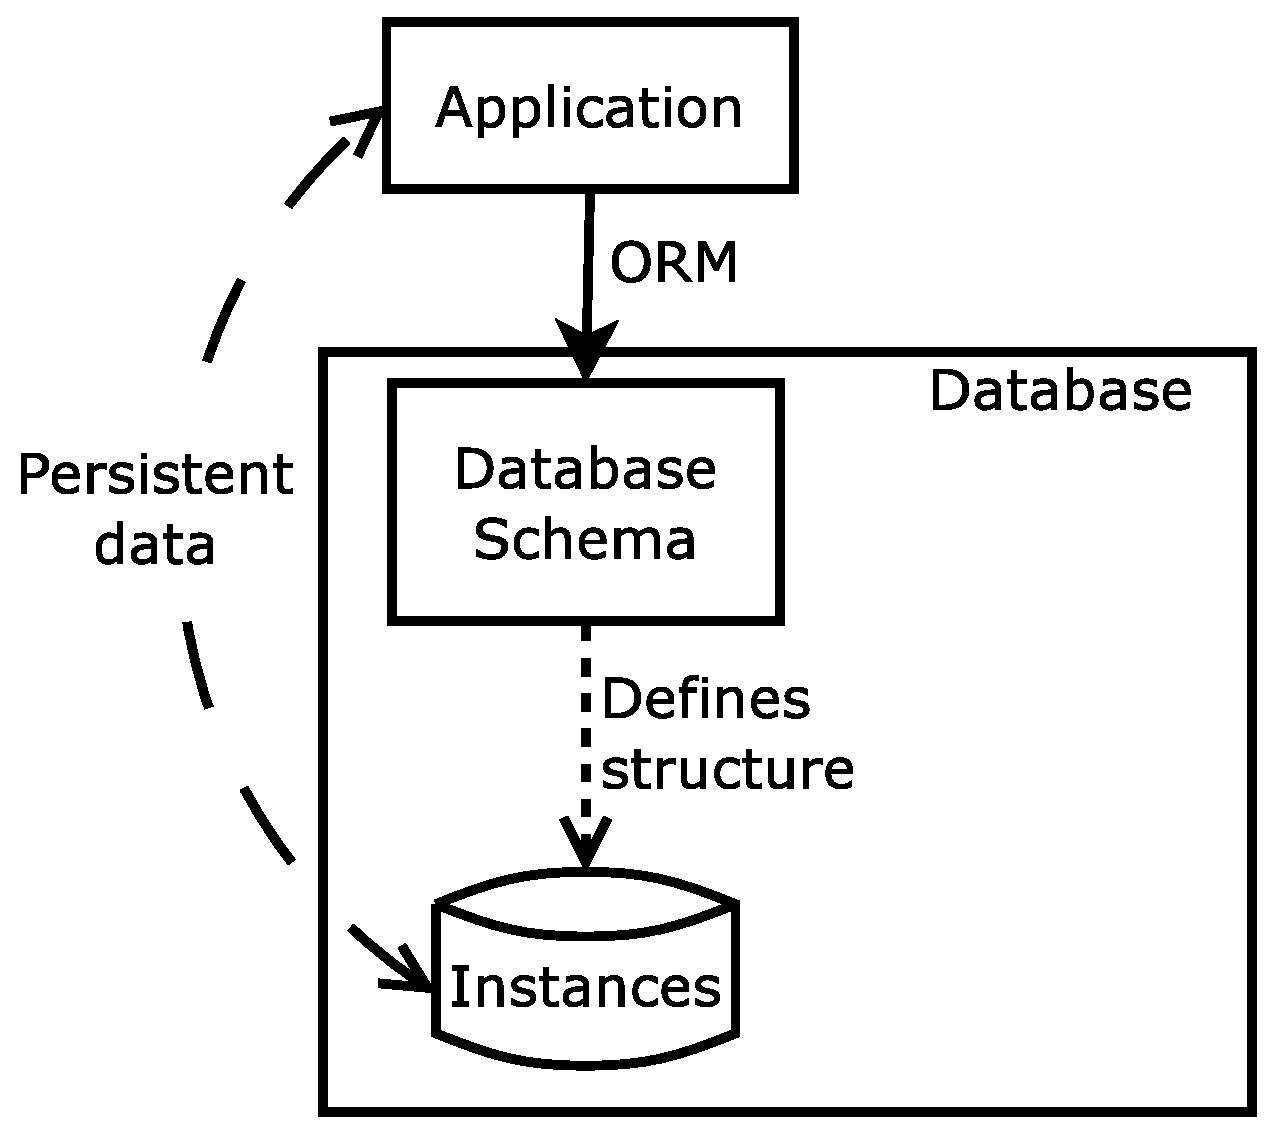
\includegraphics[scale=0.3]{./images/system}
	\caption{The model of one generation of an ORM system consists of application persistent layer and relational database for storing instances.}
\end{center}
	\label{fig:appStructure}
\end{figure}

\begin{itemize}
	\item \textbf{TODO define consistency}
	\item \textbf{TODO: $\rho(Application) = Database$ show how database is build from Application}
\end{itemize}


All important components of the domain are shown in Figure \ref{fig:appStructure}. There are three static components (static because they do not define behavior, but state of the system): an application, a database schema and stored data. Then there are four dynamic components (they define transformations between components and transition between system states): an object-relational mapping is a transformation between application and database schema, then are two components for evolution of application and of database. (To simplify the model we will consider the database schema and data are evolved by one component). Last component is the most important one - it is component which maps the evolution from application level to relational database level. We call this component evolution object-relational mapping (eORM).


There is a description of each component following. The description defines set of models of static components and dynamic components are defined as functions. There are several common parts of the model we can define in advance. The model uses a set $Labels$ which contains all possible identifiers for the model. Each model component which has a label ($label \in Labels$) is unambiguously identified in the model.

%%%%%%%%%%%%%%%%%%%




\section{Application Model}
The model represents a persistent layer of an application created using object oriented language. It means the layer is a set of instances which cooperates together. Each instance is defined according to a class - the class defines the structure and relationships of the instance. The instances are stored in the relational database in our case, therefore we define only the structure of classes in our model:
 
$$
Application = <Class*>
$$
$classes : Application \rightarrow Class*$ \\
$classes(<cs, is >) = = cs, cs \in Class* \wedge is \in Instance* $ \\ \\
$class : Label \times Application \rightarrow Class  $ \\ 
$class(l, a) = c, c \in classes(a) \wedge name(c) = l, l \in Label, a \in Application* $ \\
%TODO: variable types

The structure consist not only of classes, the structure of the application is defined by five concepts. Each concept is defined and a set of manipulating functions is define to manipulate the application model easily.

\paragraph{Class} represents a basic structural concept in the application model. It has a unique name, one or more properties and a class can be associated to other classes in the application. 
	 
$$Class = < label, Property*, Association* >$$
$name : Class \rightarrow Label$ \\
$name(< lab, props, assocs  >) = lab$ \\ \\
$properties : Class \rightarrow Property*$ \\
$properties(< lab, props, assocs  >) = props $\\ \\
$primitiveProperties : Class \rightarrow Property*$ \\
$primitiveProperties(< lab, props, assocs  >) = props', \forall p \in props' : cardinality(p) \leq 1 $\\ \\
$collectionProperties : Class \rightarrow Property*$ \\
$collectionProperties(< lab, props, assocs  >) = props', \forall p \in props' : cardinality(p) > 1 $\\ \\
$associations : Class \rightarrow Association*$ \\
$associations(< lab, props, assocs  >) = assocs $ \\ \\
$associated :  Class \times Application \rightarrow Boolean $
%TODO: variable types

\paragraph{Property} represents a feature of  a class which is can be represented as a primitive type. The property can be mandatory, can have a default value.
$$
Property = < label, AppType, DefaultValue, Cardinality, Mandatory >
$$
$name : Property \rightarrow Label$ \\
$name(< lab, t, val, n  >) = lab$ \\ \\
$type : Property \times AppType$ \\
$type(< lab, t, val, n  >) = t$ \\ \\
$cardinality : Property \rightarrow NzNat$ \\
$cardinality(< lab, t, val, n  >) = n$ \\ \\
$mandatory : Property \rightarrow Boolean $
$mandatory(<lab, t, val, n, m >) = = m $ \\ \\
$owningClass : Property \times Application \rightarrow Class $ \\
$owningClass(p, a) = c, c \in classes(a) \wedge p \in properties(c) $
%TODO: variable types

\paragraph {Association} represents a connection between two classes. It has a unique name and it contains a name of the class which is referenced by the association. The class which owns the association is consider to be a starting class of an association, referenced class is consider to be an ending class of an association. The cardinalities defines the multiplicity of the association.
$$
Association = (label, classRef, startCardinality, endCardinality)
$$
$name : Association \rightarrow Label$ \\
$name(< lab, ref, n_1, n_2  >) = lab$\\ \\
$reference : Association \rightarrow Label$ \\
$reference(< lab, ref, n_1, n_2  >) = ref$\\ \\
$startCardinality : Association \rightarrow NzNat$ \\
$startCardinality(< lab, ref, n_1, n_2  >) = n_1$\\ \\
$endCardinality : Association \rightarrow NzNat$ \\
$endCardinality(< lab, ref, n_1, n_2  >) = n_2$ \\ \\
$owningClass : Association \times Application \rightarrow Class $ \\
$owningClass(as, a) = c, c \in classes(a) \wedge as \in associations(c) $
%TODO: variable types

\paragraph{AppType} represents primitive types in the application. There are usually defined types such as String, Integer, Boolean etc. in contrast there is only one type in our model, because we focus on structural and data changes and type casting operations are not important for us. The only App-Type type is called APP-STRING.
$$
AppType = APPSTRING
$$
The types used in application model:
$$
cardinality = NzNat
$$
$$
referencesClass = label
$$
$$
startCardinality = NzNat
$$
$$
endCardinality = NzNat
$$

%%%%%%%%%%%%%%%%%%%

\section{Database Model}
The relational database consists of database schema which defines the structure of the database and data, which in our ORM system represents instances. The database is a pair:
$$
Database = <table*, row*>
$$
$table : Label \times Database \rightarrow Table $ \\
$table(l, d) = t, t \in tables(d) \wedge name(t) = l$ \\

\subsection{Database Schema Model}
The database schema model is defined by following concepts:
\paragraph{Table} represents a basic concept of database schema. It has a unique name, one or more column and it can be related to other tables in the schema by foreign keys. Rows in the table represents stored data.
$$
Table = (label, primaryKey, Column*, ForeignKey*)
$$
$name : Table \rightarrow Label $ \\
$name(< lab, pk, cols, fks  >) = lab$ \\ \\
$primaryKey : Table \rightarrow PrimaryKey $ \\
$primaryKey(< lab, pk, cols, fks  >) = pk$ \\ \\
$columns : Table \rightarrow Column* $ \\
$columns(< lab, pk, cols, fks  >) = cols$ \\ \\
$foreignKeys : Table \rightarrow ForeignKey* $ \\
$foreignKeys(< lab, pk, cols, fks  >) = fks$ 

\paragraph{Column} columns define possible data values and types which can be part of a table record.
$$
Column = (label, DbType, DefaultValue, Constraint*)
$$
$name : Column \rightarrow Label $ \\
$name(< lab, t, val, cons  >) = lab $ \\ \\
$type : Column \rightarrow DbType $ \\
$type(< lab, t, val, cons  >) = t $ \\ \\
$constraints : Column \rightarrow Constraint* $ \\
$constraints(< lab, t, val, cons  >) = cons $ \\ \\
$owningTable : Column \times Database \rightarrow Table $ \\
$constraints(c, d) = tab, tab \in tables(d) \wedge c \in columns(d) $

\paragraph{Foreign key}
$$
ForeignKey = (label, tableRef, Constraint*)
$$
$name : ForeignKey \rightarrow Label $ \\
$name(< lab, tRef, cons  >) = lab $ \\ \\
$reference : ForeignKey \rightarrow Label $ \\
$reference(< lab, tRef, cons  >) = tRef $ \\ \\
$reference : ForeignKey \rightarrow Constraint* $ \\
$reference(< lab, tRef, cons  >) = cons $ \\ \\
$owningTable : ForeignKey \times Database \rightarrow Table $ \\
$owningTable(fk, d) = tab, tab \in tables(d) \wedge fk \in foreignKeys(d) $

\paragraph{Primary key}
$$
PrimaryKey =  < label > 	
$$

\paragraph{DbType} represents primitive types in the database. There are usually defined types such as Char, Integer, Boolean etc. There is only one type defined in the model which is called DBSTRING.
$$
DbType = DBSTRING
$$

\paragraph{Constraint} there are two types of constraints defined in the model. Both constraints are column constraints - first constraint defines unique records in a column, second constraint defines non-empty columns.

\begin{center}
$Constraint = NOTNULL$ $|$ $UNIQUE $
\end{center}

\subsection{Model of Stored Data}
The representation of stored data in the relational database is based on pairs:
$$pair = < refColumn, value > | < refFK, value>$$

\textbf{TODO: primary key}
where the $refColumn$ reference a column or foreign key by its name and $value$ represents concrete value stored in the database. A row in a table is a set of pairs with reference to a concrete table:

$$row = < refTable, pair* >$$

\textbf{TODO: define consistency of rows and schema}


\section{Object-Relational Mapping}
There are defined functions for object-relational mapping used in the model. The purpose of a function is indicated in its name and should be obvious from its definition. These functions do not serve for full object-relational mapping, their purpose is to help with data evolution and its propagation from application to database.


\subsection{Mapping of Types}
The mapping of types assumes a bijection between application types and database types, otherwise these has to be additional information for type mapping. We focus on structural and data change therefore we simplify types and its mapping.

\begin{center}
$ \rho_{t} : AppType \rightarrow DbType $ \\
$ \rho_{t}(APPSTRING) = DBSTRING $
\end{center}




\subsection{Mapping of Classes}
We assume the primary key column is created automatically by database, therefore the primary key is always created with name Id and od NzNat type and properties with cardinality 0 or 1 are mapped into columns. The associations are ignored int this mapping as it is one of the partial mapping function used in eORM.

\begin{center}
$\rho_{c}: Class \rightarrow Table $ \\ 
$\rho_{c}(c,d) = table(name(c), primaryKey("Id"), \varnothing, \varnothing) $
\end{center}



\subsection{Mapping of Properties}
There are two types of properties - the first type has cardinality 1  and it is mapped to a column. A property with cardinality greater than one has to be mapped int a table not a column, thus we have a special mapping case. When the property is mandatory the $NOTNULL$ constraint is added to the column with property value. This constraint affect already stored instances a new mandatory value has to be added to each instance.

$
\rho_p : Property \times Database \rightarrow Column 
$

$\rho_p(p, d) = \begin{cases}
  \inference{ d \vdash cardinality(p) = 1 \wedge ! mandatory(p)
 \\ \wedge \exists t : t = table(name(owningClass(p)), d) 
 \\ \wedge \not instanciated(owningClass(p))
 }{\begin{gathered}
	 d \vdash columns(t) \cup column(name(p), \rho_t(type(p)), \varnothing )
\end{gathered}
 } \\ \\

  \inference{ d \vdash cardinality(p) = 1 \wedge mandatory(p)
 \\ \wedge \exists t : t = table(name(owningClass(p)), d)}{\begin{gathered}
 	d \vdash columns(t) \cup column(name(p), \rho_t(type(p)), NOTNULL ) \\
 	
 	
\end{gathered}
} 
\\ \\
 
 \inference{d \vdash cardinality(p) > 1 \wedge ! mandatory(p) \\ \wedge \exists t : t = table(name(owningClass(p)), d)}{\begin{gathered}d \vdash  table(name(p), primaryKey("Id"), column("value", \rho_t(type(p))), \\ foreignKey(name(p), name(owningClass(p)), \varnothing) \\
 
\end{gathered}}
\\ \\

 \inference{d \vdash cardinality(p) > 1 \wedge mandatory(p) \\ \wedge \exists t : t = table(name(owningClass(p)), d) }{\begin{gathered}d \vdash  table(name(p), primaryKey("Id"), \\ column("value", \rho_t(type(p)), NOTNULL), \\ foreignKey(name(p), name(owningClass(p)), NOTNULL)
	 \end{gathered}}
 \end{cases}$

\subsection{Mapping of Associations}
A association is mapped into database as a foreign key in table representing associating class or an association can be mapped as a coupling table in case the association cardinality is M:N or 1:N.

$
\rho_a(a,d) = \begin{cases}
 \inference{d \vdash startCardinality(a) = 0 \\ \wedge \exists t : t = table(name(owningClass(p)), d) \\ \wedge \exists u : u = table(reference(a)), d)}{d \vdash 
 \begin{gathered}
 foreignKeys(u) \\ \cup foreignKey(name(a), name(t),  \varnothing) 
 \end{gathered}
 }
  \\ \\
 \inference{d \vdash startCardinality(a) = 1 \\ \wedge \exists t : t = table(name(owningClass(p)), d) \\ \wedge \exists u : u = table(reference(a)), d)}{\begin{gathered} d \vdash 
foreignKeys(u) \\ \cup  foreignKey(name(a), name(t),  NOTNULL) \\
\end{gathered}
} \\ \\
 
  \inference{d \vdash  startCardinality > 1 \\ \wedge \rho(owningClass(p)) \in tables(d) \wedge \rho(reference(a)) \in tables(d)}{
  \begin{gathered} d \vdash 
 table(name(a), pk("Id"), \varnothing, \\ foreignKey(owningClass(a),owningClass(a), NOTNULL) \\ foreignkey(reference(a), reference(a), NOTNULL)) 
  \end{gathered}}  
 \end{cases}
$
\textbf{TODO: check + add cardinalities/images and split(?), data in NOTNULL}

The new foreign key can cause inconsistency of the system when added to a table which contains data. This case is not handled by the mapping function above. We have to extend the function definition of a feature that allows the mapping between the data in both tables. The mapping is a function:
$$f_m : Property \rightarrow Instance \times Instance $$
%TODO handle instances




\section{Data Evolution in ORM System}
The Object-Relational system consist of an application and a database. The system has to be in consistent state, therefore the evolution of application has to be propagated correctly into database. Each evolution operation consist of two parts - applying evolution operation on application and on database. The mapping of the evolution change is called extended Object-Relational Mapping (eORM). The eORM mapping helps to assure consistency of the system by transforming application evolution into database schema and data. Each eORM function applied on an ORM system produces a new generation of the system. If the function cannot be applied on a system the system cannot be evolved by the function. 

The state of a system is called generation and transformation from one state to another is called evolution. The state of the system defines a context for each evolution and it determines if the evolution is successful or not. 

\begin{figure}
\begin{center}
	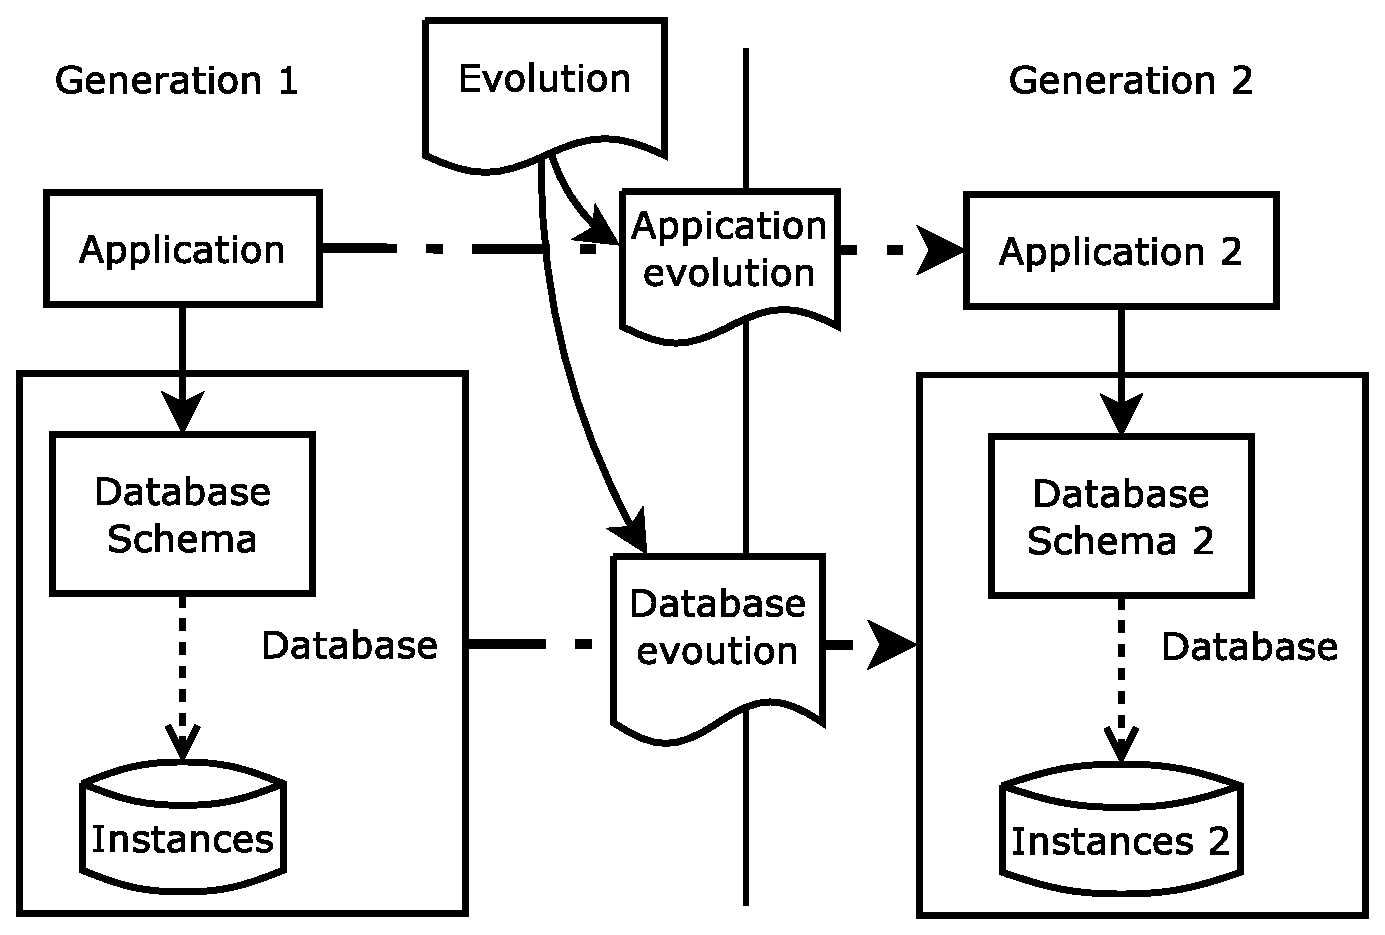
\includegraphics[scale=0.4]{./images/evolution_simple}
	\caption{The evolution of data changes the system on all levels}
\end{center}
	\label{fig:evolution}
\end{figure}

This section defines eORM for each trivial operation evolving application from \ref{sec:appEvolution}, moreover there are described more complex cases of evolution. 

\begin{itemize}
	\item \textbf{TODO show how a whole system is evolved}
	\item \textbf{TODO state monade}
\end{itemize}


\subsection{Evolution of Application}
\label{sec:appEvolution}

The evolution is defined as a set of operations which change structure of an application. The definition of an operation consists of two parts - a conditions of operation feasibility and operation impact on the application structure. We decide to use following transcription:

$$
operation = \inference{conditions$ $of$ $feasibility}{impact$ $on$ $application$ $structure}
$$
If the conditions of feasibility are not met, the operation cannot impact the application structure.
%TODO monade


\subsubsection{Application Creation}
$$addClass: Class \times Application \rightarrow Application $$

$
addClass(c, a) = \inference{\forall s \in classes(A) : name(s) \neq name(c)}
{classes(a) \cup c}
$

$$AddProperty : Label \times Property \times Application \rightarrow Application $$

$
AddProperty(l, p, a) = \inference{\exists c \in classes(a) : name(c) = l \\ \wedge \forall q \in  properties(p) : name(q) \neq name(p)}{properties(c) \cup p }
$
$$AddAssociation : Label \times Association \times Application \rightarrow Application $$
$
AddAssociation(l, s, a) = \inference{\forall f \in associations(a) : name(f) \neq name(s) \\ \wedge \exists c \in classes(a) : name(c) = l \\ \wedge \exists k \in classes(a) : name(k) = reference(s) }{associations(c) \cup s}
$

\subsubsection{Application Deconstruction}
$$RemoveClass: Label \times Application \rightarrow Application $$
$
RemoveClass(q, a) = \inference{\exists c \in classes(a) : name(c) = q \\
\wedge not$ $instantiated(c) = \varnothing \wedge not$ $associated(c)}{classes(a) \setminus c }
$

$$RemoveProperty: Label \times Label \times Application \rightarrow Application $$

$
RemoveProperty(l_c, l_p, a) = \inference{\exists c \in classes(a) : name(c) = l_c \\ \wedge \exists p \in properties(c) : name(p) = l_p}{properties(c) \setminus p }
$

$$RemoveAssociation : Label \times Labels \times Application \rightarrow Application $$

$
RemoveAssociation(l_c, l_a, a) = \inference{\exists c \in classes(a) : name(c) = l_c \\ \wedge \exists s \in associations(c) : name(s) = l_a }{associations(c) \setminus s}
$

\subsubsection{Application Alternation}
\paragraph{Rename}
\paragraph{Change Cardinality}
\paragraph{Copy Property}


\subsection{ORM System Evolution}
Creational operations does not have impact on stored data they change the structure of the application and database by adding new objects into model.

\subsubsection{Creation of a System}
\paragraph{Add Class}

$
\Phi_{addClass}(c, d) = \inference{d \vdash \forall t \in tables(d) : name(t) \neq name(\rho(c)) \\
	\forall a \in associations(c), \exists u \in  tables(d) : reference(a) = name(u) 
}{
\begin{gathered}
d \vdash  tables(d) \cup \rho(c) \cup \rho(collectionProperties(c)) \\ \cup \rho(associations(c))
\end{gathered}
}
$
\paragraph{Add Property}
$
\Phi_{addProperty}(p, d) = \begin{cases}
\inference{d \vdash \exists t \in tables(d) : name(t) = name(owningClass(p)) \wedge (! mandatory(p) \vee ! instantiated(owningClass(p))}{d \vdash \rho(p,d)} 
\\ \\ 
\inference{d \vdash \exists t \in tables(d) : name(t) = name(owningClass(p)) \wedge mandatory(p) \wedge instantiated(owningClass(p)) \wedge cardinality(p) \leq 1}{d \vdash \rho(p,d) \wedge \forall r \in data(d), reference(r) = t : pair(r) \cup pair(name(p), defaultValue(p))} 
\\ \\
\inference{d \vdash \exists t \in tables(d) : name(t) = name(owningClass(p)) \wedge mandatory(p) \wedge instantiated(owningClass(p)) \wedge cardinality(p) \leq 1}{\begin{gathered}
 \rho(p,d) \wedge \forall r \in row(owningClass(p)) : data(d)\\ \cup row(name(p), pair("value", defaultValue(p)), \\ pair(name(p), value(primaryKey(r))) 
\end{gathered}
} 

\end{cases}
$

\paragraph{Add Association}
$
\Phi_{AddAssociation}(a, d) = \inference{d \vdash \exists t_s, t_t \in tables(d) : name(t_s) = name(owningClass(a)) \\ \wedge name(t_t) = reference(a) \\ \wedge \not \exists f \in foreignKeys(t_t) : name(f) = name(a) }{d \vdash \rho(a,d)}
$


\subsubsection{Deconstruction of a System}
\paragraph{Remove Class}
$
\Phi_{removeClass}(c,d) = \inference{d \vdash \rho(c) \in tables(d) \\ \wedge \not \exists r \in data(d) : owningTable(r) = \rho(c) \\ \not \exists j \in tables(d), f \in foreignKeys(j) : reference(f) = \rho(c)  }{d \vdash tables(d) \setminus \rho(c)}
$
%TODO remove by label

\paragraph{Remove Property}
$
\Phi_{removeProperty}(l_c, l_p, d) = \begin{cases}
 \inference{d \vdash \exists t \in tables(d) : name(t) = l_c \\ \wedge \exists c \in columns(t) : name(c) = l_p  }{d \vdash
columns(t) \setminus c
} \\ \\
  \inference{d \vdash \exists t \in tables(d) : name(t) = l_c \\ \wedge \not \exists c \in columns(t) : name(c) = l_p \\ \wedge \exists u \in tables(d) : name(u) = l_p }{d \vdash tables(d) \setminus u }
 \end{cases}
$

\paragraph{Remove Association}
$
\Phi_{removeAssociation}(l_c, l_a, d) = d \vdash \begin{cases}
 \inference{\exists t \in tables(d) : name(t) = l_c 
 \\ \wedge \exists f \in foreignKeys(t) : name(f) = l_a 
 \\ \wedge not containsData(t)}{d \vdash foreignKeys(t) \setminus f }
 \\ \\
 \inference{\exists t \in tables(d) : name(t) = l_a 
 \\ \wedge \exists f \in foreignKeys(t) : name(f) = l_c
 \\ \wedge not containsData(t)}{d \vdash tables(d) \setminus t}
 \end{cases}
$

\subsubsection{Altering of a System}	



\end{document}
